\chapter{Metodo del simplesso}
\section{Cosa è il metodo del simplesso?}
Il metodo del simplesso è un algoritmo iterativo utilizzato per risolvere problemi di programmazione lineare. Nel caso medio il tempo computazionale è lineare, nel caso peggiore può risultare esponenziale.


\section{Definizioni geometriche}
\subsection{Frontiera del vincolo}
La frontiera del vincolo rappresenta l'insieme dei punti limite che separano lo spazio delle soluzioni in base al rispetto o alla violazione di un determinato vincolo

\begin{figure}[H]
    \centering
    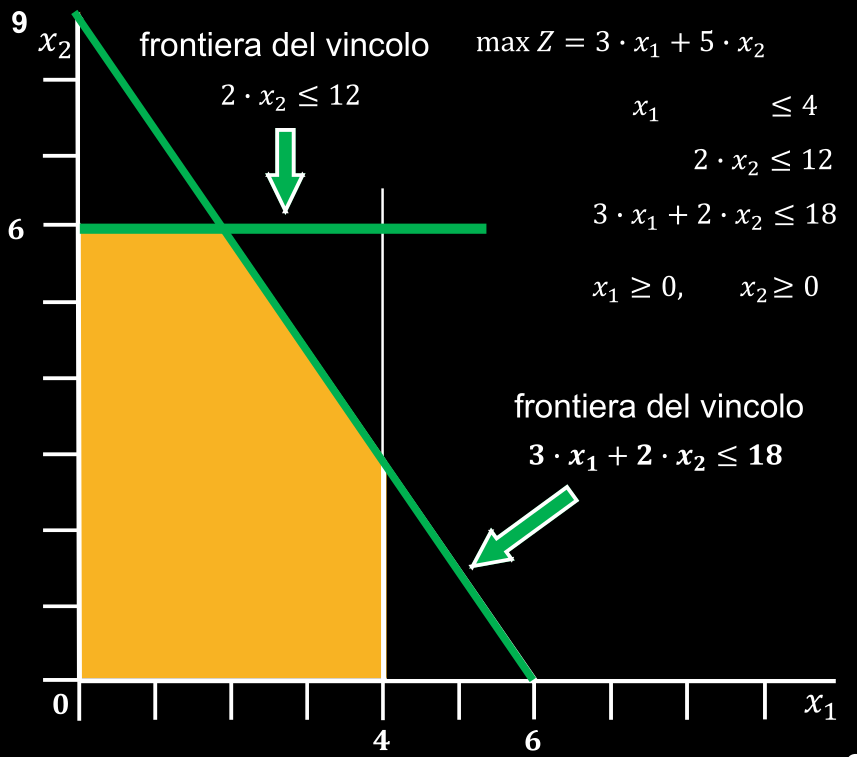
\includegraphics[scale=0.3]{Immagini/Frontiera del vincolo.png}
    \caption*{Esempio di frontiera}
\end{figure}

\subsection{Vertici}
\subsubsection{Definizione generale}
I vertici sono punti che risiedono all'intersezione di coppie di frontiere di vincoli

\begin{figure}[H]
    \centering
    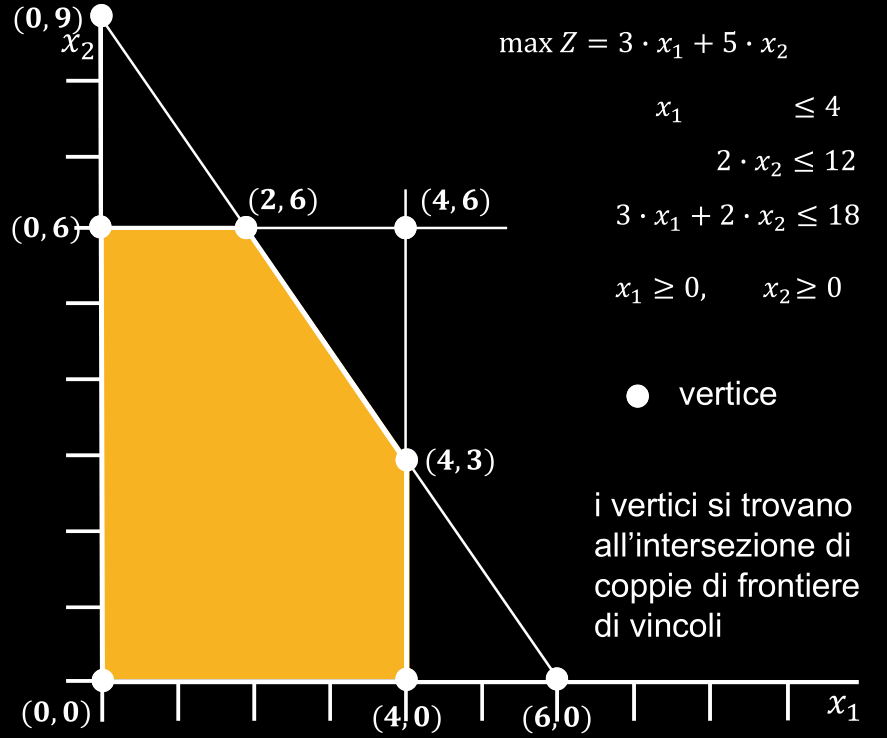
\includegraphics[scale=0.25]{Immagini/Vertici.png}
\end{figure}

\subsubsection{Vertice ammissibile}
Un vertice si dice \textbf{ammissibile} quando la soluzione del sistema di equazioni di frontiera \uline{soddisfa tutti i vincoli del problema}

\textbf{Geometricamente} il punto si trova esattamente all'interno o sul bordo della regione ammissibile

\begin{figure}[H]
    \centering
    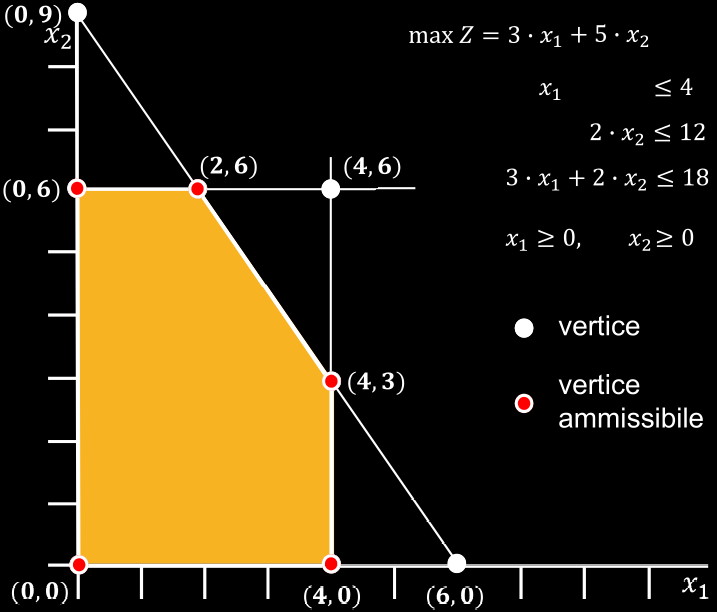
\includegraphics[scale=0.37]{Immagini/Vertice ammissibile.png}
\end{figure}

\subsubsection{Vertice non ammissibile}
Un vertice si dice \textbf{non ammissibile} quando la soluzione ottenuta dall'intersezione di alcune equazioni di frontiera viola almeno uno dei vincoli rimanenti del problema

\textbf{Geometricamente} il punto si trova all'esterno della regione ammissibile.

\begin{figure}[H]
    \centering
    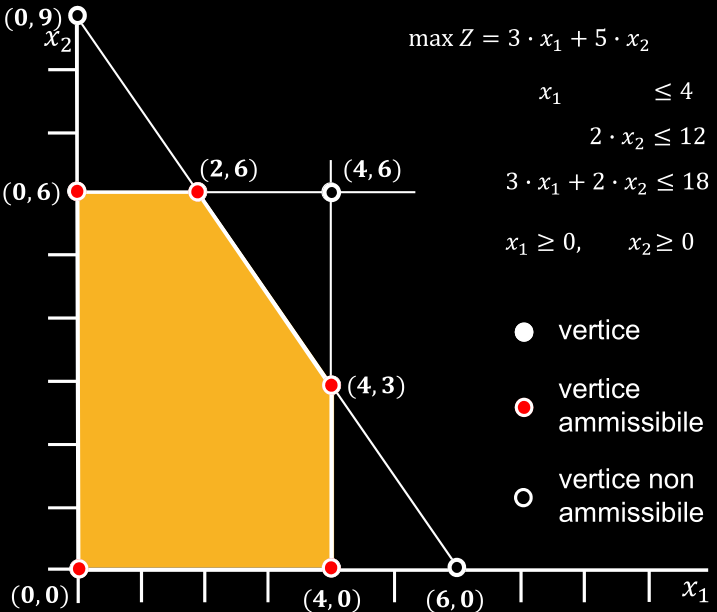
\includegraphics[scale=0.37]{Immagini/Vertice non ammissibile.png}
\end{figure}

\newpage
\subsubsection{Vertici adiacenti}
Per ogni problema di PL con $n$ variabili decisionali, due vertici sono detti \textbf{adiacenti} se \uline{condividono $n-1$ frontiere di vincoli}.

\begin{center}
    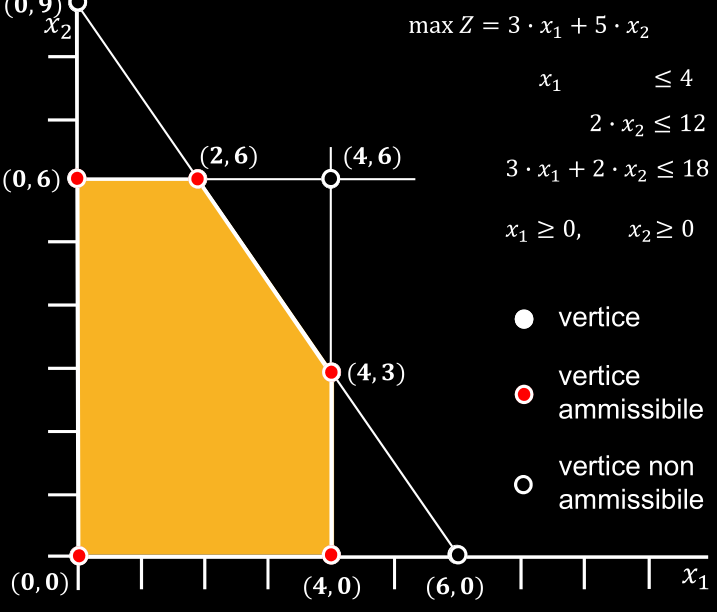
\includegraphics[scale=0.37]{Immagini/Vertici adiacenti.png}

    \vspace{0.5cm}

    \begin{tabular}{|c|c|}
        \hline \textbf{Vertice Ammissibile} & \textbf{Vertici Ammissibili Adiacenti} \\ \hline
        $(0,0)$ & $(0,6);(4,0)$ \\ \hline
        $(0,6)$ & $(2,6);(0,0)$ \\ \hline
        $(2,6)$ & $(4,3);(0,6)$\\ \hline
        $(4,3)$ & $(4,0);(2,6)$\\ \hline
        $(4,0)$ & $(0,0);(4,3)$\\ \hline
    \end{tabular}
\end{center}


\subsection{Spigolo}


Due vertici adiacenti sono collegati da un segmento che giace sull'intersezione delle frontiere dei vincoli condivisi. Questo segmento viene indicato con il termine \textbf{spigolo} della regione ammissibile

\begin{figure}[H]
    \centering
    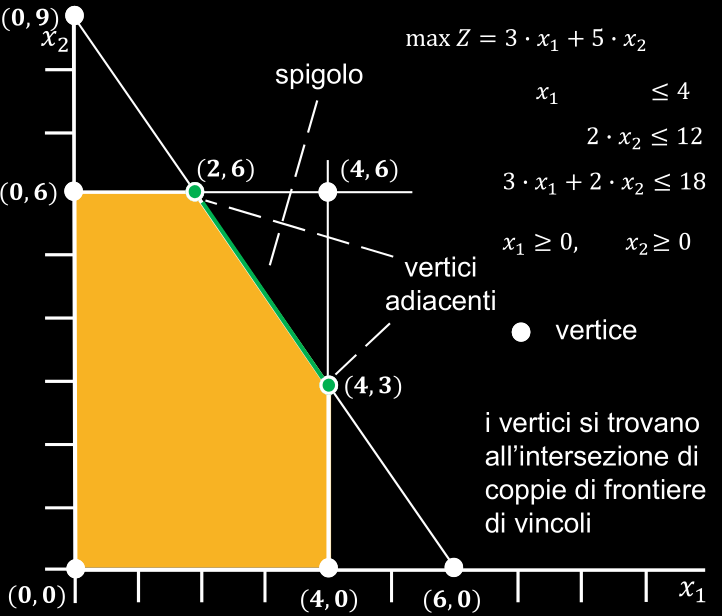
\includegraphics[scale=0.4]{Immagini/Spigolo.png}
\end{figure}

\section{Test di ottimalità}
Si consideri ogni problema di PL tale da ammettere almeno una soluzione ottimale.

\begin{center}
    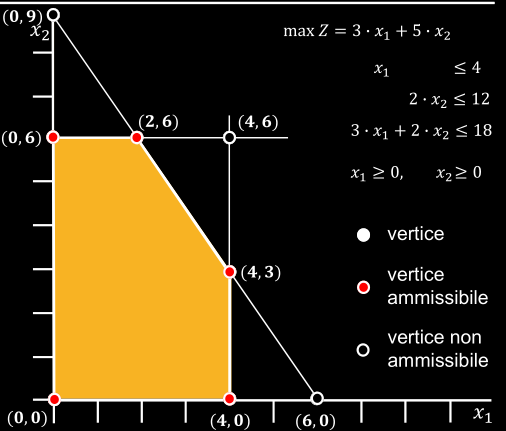
\includegraphics[scale=0.5]{Immagini/Test ottimalità 1.png}
\end{center}

Se una soluzione vertice non ammette soluzioni vertice a lei adiacenti con valore della funzione obiettivo $Z$ migliore, allora la soluzione in questione è ottimale

\begin{center}
    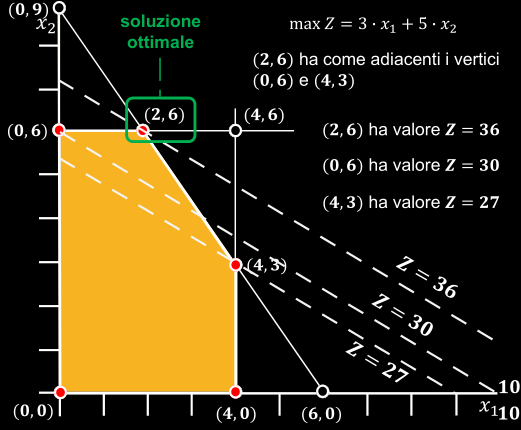
\includegraphics[scale=0.5]{Immagini/Test ottimalità 2.png}
\end{center}

\newpage
\section{Concetti chiave}
\subsection{Concetto chiave 1}
Il metodo del simplesso ispeziona solo le soluzioni ammissibili corrispondenti a vertici.

Per ogni problema di PL che ammette almeno una soluzione ottimale, trovarne una, richiede di trovare solamente il vertice ammissibile cui compete il miglior valore della funzione obiettivo.

Dato che il numero di soluzioni ammissibili è generalmente infinito, ridurre il numero di soluzioni da ispezionare ad un numero finito e piccolo è una semplificazione notevole. La sola restrizione è che il problema possegga vertici ammissibili, cioò è garantito dal fatto che la regione ammissibile è limitata.

\begin{center}
    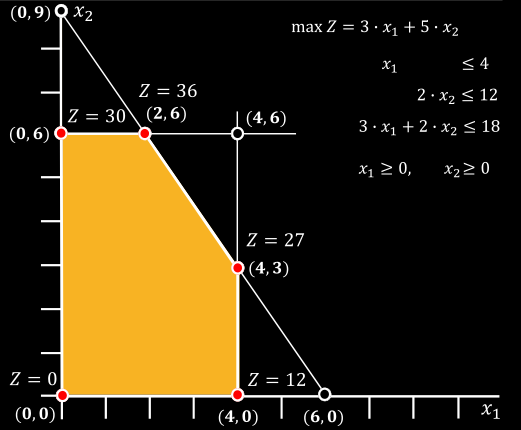
\includegraphics[scale=0.5]{Immagini/Concetto chiave 1.png}
\end{center}

\subsection{Concetto chiave 2}
Il metodo del simplesso è un algoritmo iterativo con la seguente struttura:
\begin{enumerate}
    \item \textbf{Inizializzazione:} Scelta di una soluzione
    \item \textbf{Test di ottimalità:} La soluzione è ottimale?
    \begin{itemize}
        \item \textbf{NO:} Tornare al punto 1 per trovare una soluzione migliore di quella corrente
        \item \textbf{SI:} Termina algoritmo
    \end{itemize}
\end{enumerate}

\begin{center}
    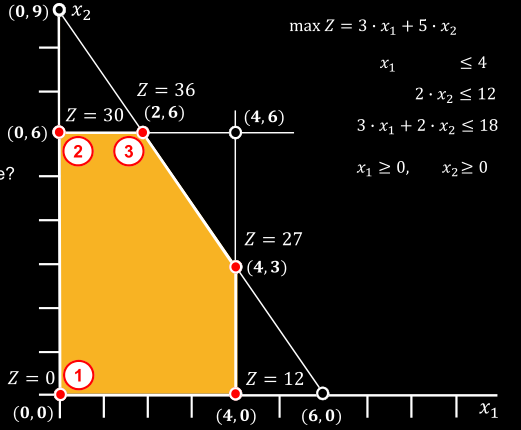
\includegraphics[scale=0.5]{Immagini/Concetto chiave 2.png}
\end{center}

\subsection{Concetto chiave 3}
Quando sia possibile, l'inizializzazione del metodo del simplesso selezione l'origine (i valori di tutte le variabili di decisione vengono posti uguali a 0) come soluzione iniziale.

Se vi sono molte variabili decisionali, tali da rendere il metodo grafico per scegliere la soluzione iniziale, scegliere l'origine evita di ricorrere a procedure algebriche per determinare la soluzione iniziale del metodo del simplesso. La soluzione nulla (origine) potrebbe però essere una soluzione non ammissibile. Se questo accade, vengono usate procedure specifiche per la scelta della soluzione iniziale.

\begin{center}
    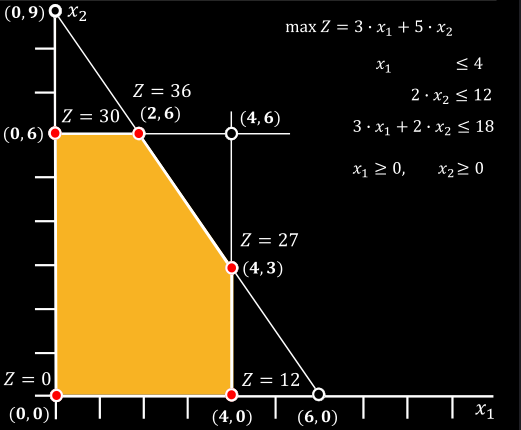
\includegraphics[scale=0.5]{Immagini/Concentto chiave 3.png}
\end{center}

\subsection{Concetto chiave 4}
Dato un vertice, è più vantaggioso, in termini computazionali, acquisire informazioni sui vertici a lui adiacenti di quanto non sia per i vertici a lui non adiacenti.

Ad ogni iterazione, se l'algoritmo si sposta dal vertice corrente, verso un vertice con valore migliore della funzione obiettivo, lo fa per muoversi in un vertice a lui adiacente. Nessuna altra soluzione viene considerata.

Pertanto, l'intero cammino, che partendo dalla soluzione iniziale raggiunge quella ottimale, attraversa spigoli della regione ammissibile.

\begin{center}
    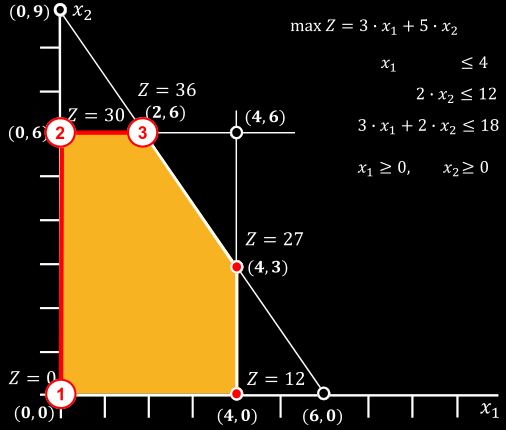
\includegraphics[scale=0.5]{Immagini/Concetto chiave 4.png}
\end{center}

\subsection{Concetto chiave 5}
A partire dal vertice corrente, il metodo del simplesso valuta i vertici ad esso adiacenti, ma non lo fa calcolando il valore della funzione obiettivo per ognuno di essi.

Il metodo del simplesso valuta e compara i tassi di miglioramento della funzione obiettivo $Z$ lungo la direzione degli spigoli che conducono dal vertice corrente ai vertiici adiacenti.

Tra i vertici adiacenti con un tasso di miglioramento positivo per la funzione obiettivo $Z$, il metodo del simplesso sceglie di muoversi lungo lo spigolo cui compete il massimo valore di incremento.

Il vertice selezionato diviene il nuovo vertice corrente.

\begin{center}
    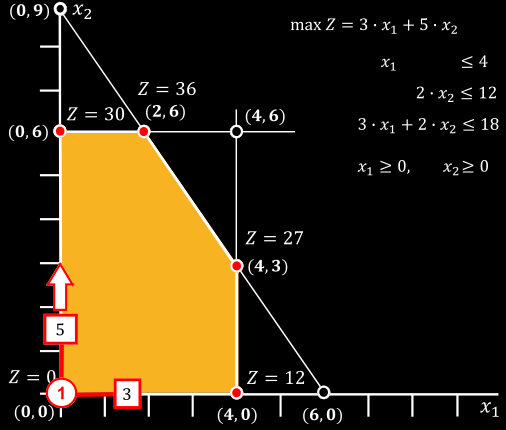
\includegraphics[scale=0.5]{Immagini/Concetto chiave 5.png}
\end{center}

\subsection{Concetto chiave 6}
Il \textbf{concetto chiave 5} descrive come il metodo del simplesso esamina gli spigoli che emanano dal vertice corrente.

L'ispezione di uno spigolo consente di identificare rapidamente il tasso di miglioramento di $Z$ che si otterrebbe muovendosi lungo di esso verso la soluzione adiacente all'altro estremo.

Un tasso di miglioramento positivo per $Z$ significa che il vertice adiacente è una soluzione migliore della soluzione corrente. Un tasso negativo implica che il vertice adiacente è una soluzione peggiore della soluzione corrente.

Il \textbf{Test di ottimalità} consiste nel verificare se esiste uno spigolo con tasso positivo di miglioramento. Se tale condizione non è soddisfatta allora la soluzione corrente è ottimale.

\begin{center}
    \begin{minipage}{0.45\textwidth}
        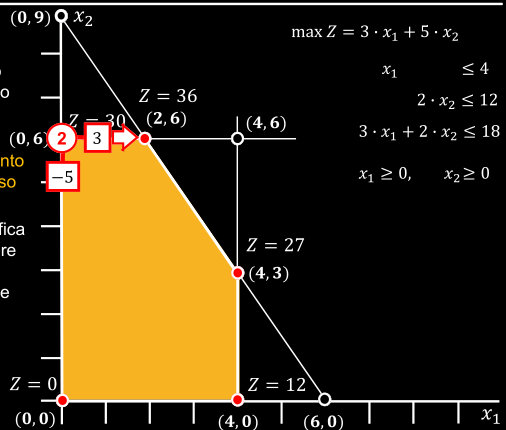
\includegraphics[scale=0.45]{Immagini/Concetto chiave 6_1.png}
    \end{minipage}
    \hfil
    \begin{minipage}{0.45\textwidth}
        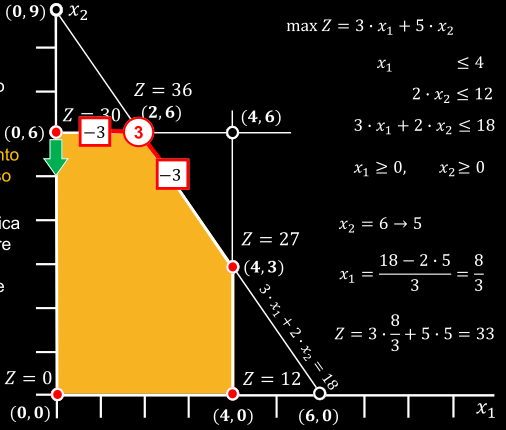
\includegraphics[scale=0.45]{Immagini/Concetto chiave 6_2.png}
    \end{minipage}
\end{center}

\section{Definizioni algebriche}
\subsection{Idea di partenza}
Fino ad ora abbiamo introdotto i concetti geometrici necessari per parlaredel metodo del simplesso, ora passeremo al tradurre la procedura geometrica in una procedura algebrica.

La procedura algebrica si basa sulla risoluzione di un sistema di equazioni lineari.

Pertanto, il primo passo da compiere per tradurre la procedura geometrica in procedura algebrica richiede di traddure i vincoli funzionali di diseguaglianza in vincoli funzionali di eguaglianza. I vincoli di non negatività vengono mantenuti invariati in quanto la loro trattazione viene effettuata in maniera separata

\subsection{Variabili slack}
Convertire i vincoli di diseguaglianza in vincoli di ugualianza viene effettuato introducendo il concetto di \textbf{variabile slack}

\begin{center}
    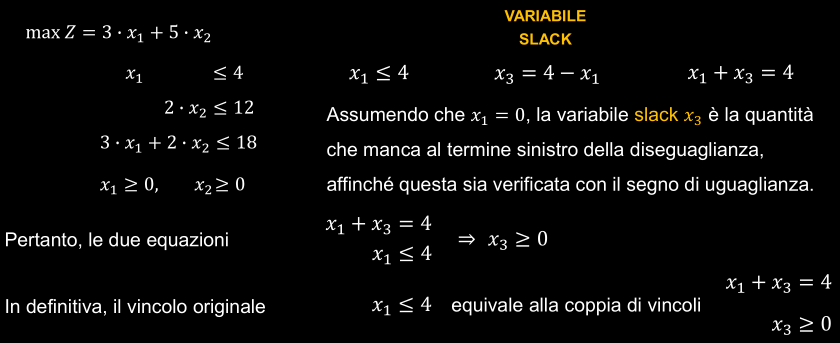
\includegraphics[scale=0.6]{Immagini/Variabile slack.png}
\end{center}

\subsection{Forma aumentata}
Introducendo una variabile slack per ognuno dei restanti vincoli del problema di programmazione lineare in forma originale otteniamo la seguente formulazione equivalente

\begin{center}
    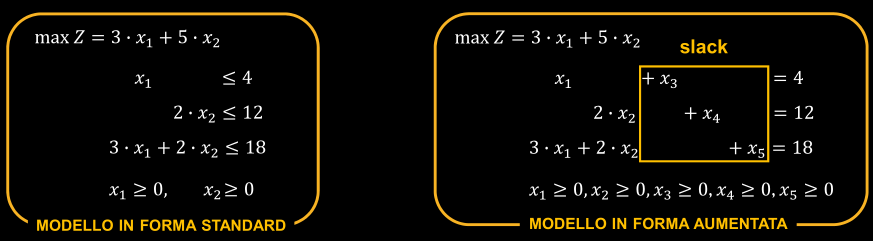
\includegraphics[scale=0.6]{Immagini/Forma aumentata.png}
\end{center}

\newpage
\subsubsection{Slack pari a 0}
Se la \textbf{variabild slack di un vincolo assume valore zero}, allora la soluzione corrispondente giace sulla frontiera del vincolo della forma originale. (Il vincolo corrispondente della forma originale è verificato come ugualianza)

\begin{center}
    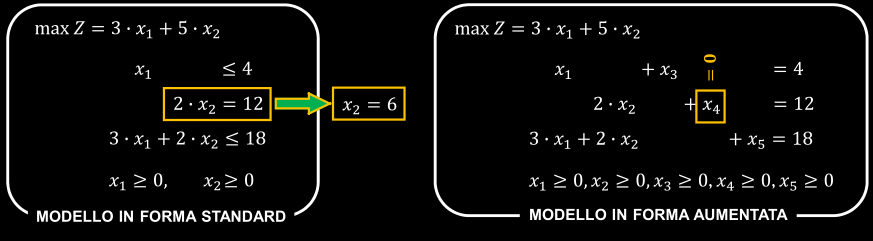
\includegraphics[scale=0.6]{Immagini/Slack=0.png}
\end{center}

\subsubsection{Slack positive}
Se la \textbf{variabile slack di un vincolo assume valore positivo}, allora la soluzione corrispondente giace sulla frontiera del vincolo della forma originale, vale a dire la soluzione appartiene alla regione ammissibile (è interna alla regione ammissibile)

\begin{center}
    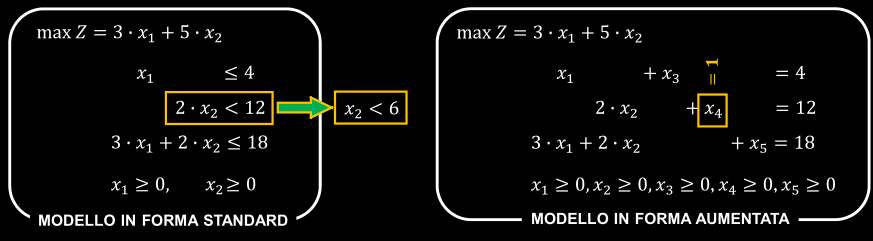
\includegraphics[scale=0.6]{Immagini/Slack >.png}
\end{center}

\subsubsection{Slack negative}
Se la \textbf{variabile slack di un vincolo assume valore negativo}, la soluzione corrispondente appartiene al semipiano non ammissibile della frontiera del vincolo della forma originale, vale a dire la soluzione non appartiene alla regione ammissibile.

\begin{center}
    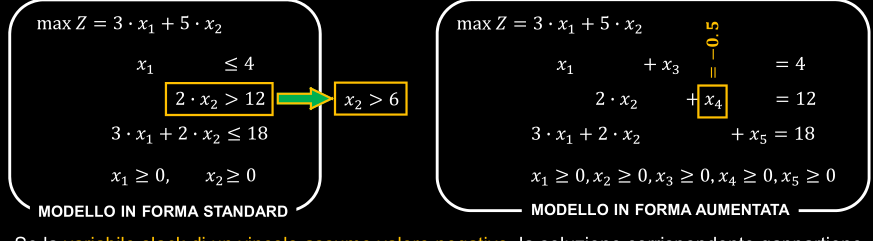
\includegraphics[scale=0.6]{Immagini/Slack <.png}
\end{center}

\newpage
\subsection{Soluzione aumentata}
Si definisce soluzione aumentata, una soluzione del modello in forma originale (valori delle variabili di decisione) che viene aumentata tramite i corrispondenti valori delle variabili di slack

\begin{center}
    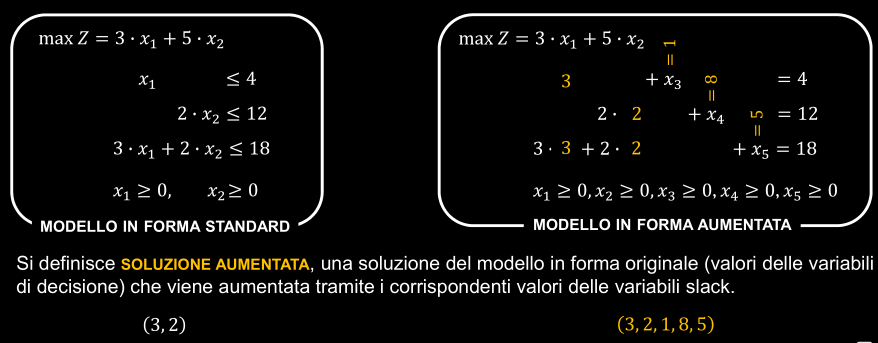
\includegraphics[scale=.6]{Immagini/Saluzione aumentata.png}
\end{center}

\subsection{Soluzione di base}
Si definisce soluzione di base, un vertice del modello in forma aumentata.

\begin{center}
    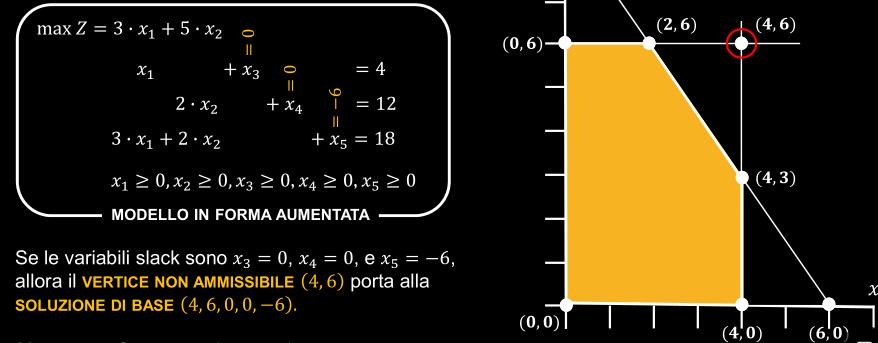
\includegraphics[scale=0.6]{Immagini/Soluzione di base.png}
\end{center}

\newpage
\subsubsection{Soluzione di base ammissibile}
Si dice soluzione di base ammissibile una soluzione associata a un vertice ammissibile che venga aumentata.

\begin{center}
    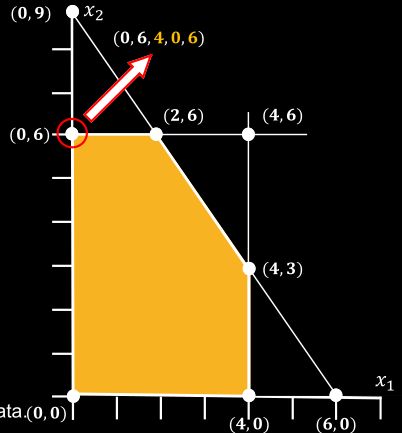
\includegraphics[scale=.5]{Immagini/Soluzione di base ammissibile.png}
\end{center}

\subsection{Variabili di base}
I termini soluzione di base e soluzione ammissibile sono molto importanti ed è quindi necessario chiarirne le proprietà algebriche.

Due variabili poste a 0, per esempio:
$$x_1 = 0,\ x_4=0$$ vengono dette \textbf{variabili non di base}.

La soluzione del sistema lineare per le 3 variabili restanti, dette \textbf{variabili di base}
$$
x_2=6,\ x_3=4,\ x_5=6
$$
porta alla seguente \textbf{soluzione di base}
$$
x_1=0,\ x_2=6,\ x_3=4,\ x_4=0,\ x_5=6
$$

Il modello in forma aumentata consiste di 5 variabili (2 decisionali e 3 slack) e di 3 equazioni.

Abbiamo a disposizione $2=(5-3)$ \textbf{gradi di libertà} per risolvere il sistema lineare.

\begin{center}
    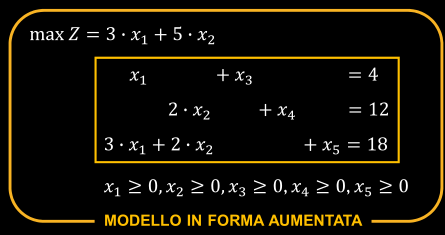
\includegraphics[scale=0.7]{Immagini/Variabili di base e non.png}
\end{center}

\subsection{Proprietà delle soluzioni di base}
\begin{enumerate}
    \item Una variabile può essere una \textbf{variabile di base} o una \textbf{variabile non di base}
    \item Il numero delle variabili di base eguaglia il numero dei vincoli funzionali (equazioni).

    Pertanto, il numero delle variabili non di base eguaglia il numero totale delle variabili meno il numero dei vincoli funzionali.
    
    \item Le variabili non di base vengono poste a zero
    \item I valori delle variabili di base sono ottenuti come risoluzione simultanea del sistema di equazioni lineare (vincoli funzionali in forma aumentata).

    L'insieme delle variabili di base viene spesso riferito con il termine di \textbf{base}

    \item Se le variabili di base soddisfano i vincoli di non negatività, la soluzione di base è una soluzione ammissibile di base
\end{enumerate}

\subsection{Soluzione di base ammissibile}
Consideriamo la soluzione di base $(0,6,4,0,6)$.

Questa soluzione viene ottenuta aumentando la soluzione corrispondente al vertice ammissibile $(0,6)$

\begin{center}
    \begin{minipage}{0.45\textwidth}
        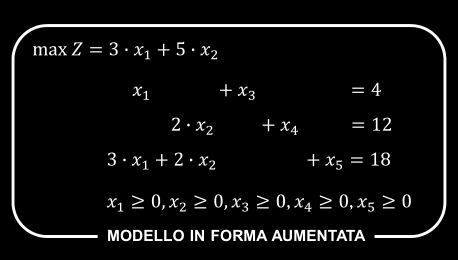
\includegraphics[scale=0.5]{Immagini/Soluzione di base ammissibile_1.png}
    \end{minipage}
    \hfil
    \begin{minipage}{0.45\textwidth}
        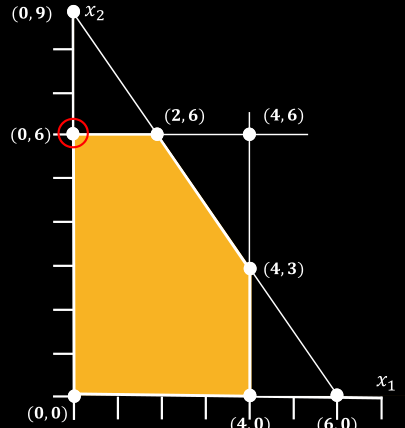
\includegraphics[scale=0.5]{Immagini/Soluzione di base ammissibile_2.png}
    \end{minipage}
\end{center}

Comunque, un modo alternativo per ottenere la stessa soluzione, consiste nel fare in modo che le due variabili $x_1$ e $x_4$ siano \textbf{variabili non di base}, e pertanto nel porne i rispettivi valori a zero $(x_1=0,\ x_4=0)$.

Se $x_1=0$ e $x_4=0$ la soluzione del \textbf{sistema lineare} è

$$
    x_1=0,\ x_2 = 6,\ x_3=4,\ x_4=0,\ x_5=6
$$

che determina il valore delle tre \textbf{variabili di base}.

Le tre \textbf{variabili di base} $x_2,x_3,x_5$ sono non negative, pertanto la \textbf{soluzione di base} $\mathbf{(0,6,4,0,6)}$ è una \textbf{soluzione di base ammissibile}

\begin{center}
    \begin{minipage}{0.45\textwidth}
        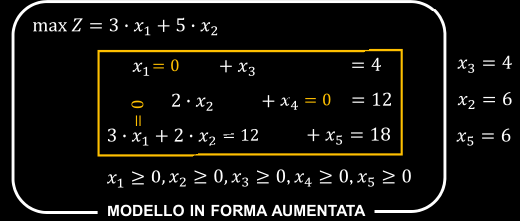
\includegraphics[scale=0.5]{Immagini/Soluzione di base ammissibile_3.png}
    \end{minipage}
    \hfill
    \begin{minipage}{0.45\textwidth}
        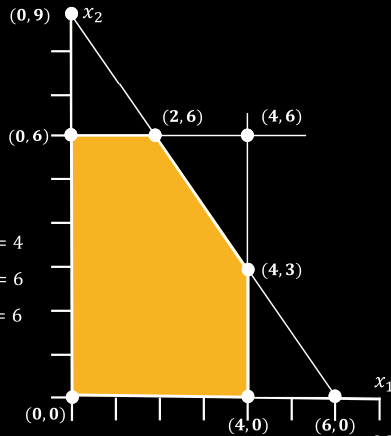
\includegraphics[scale=0.5]{Immagini/Soluzione di base ammissibile_4.png}
    \end{minipage}
\end{center}

\subsection{Soluzioni di base ammissibili adiacenti}

Così come certe coppie di vertici ammissibili sono tra loro adiacenti, le corrispondenti coppie di \textbf{soluzioni di base ammissibili} sono tra loro adiacenti.

Due \textbf{soluzioni di base ammissibili} sono adiacenti se sono caratterizzate dal condividere le stesse \textbf{variabili non di base} eccetto una. Questo implica che tutte le loro \textbf{variabili di base} sono uguali eccetto una, anche se esse possono assumere valori differenti.

Conseguentemente, muoversi dalla \textbf{soluzione di base ammissibile} corrente ad una soluzione ad essa adiancente implica che una \textbf{variabile non di base} divenga una \textbf{variabile di base} e che una \textbf{variabile di base} divenga una \textbf{variabile non di base} (il che richiede di aggiustare i valori delle variabili di base per garantire che il sistema lineare di equazioni sia ancora soddisfatto)

Al fine di illustrare \textbf{soluzioni di base ammissibili} che siano adiacenti, consideriamo la seguente coppia di vertici ammissibili $(0,0)$ e $(0,6)$.

\begin{center}
    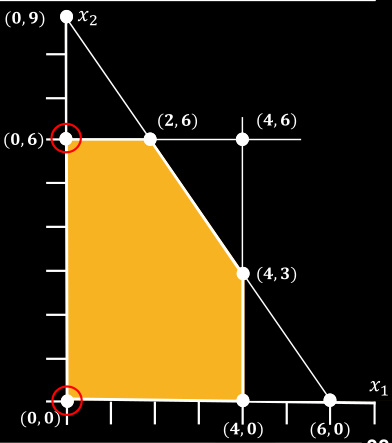
\includegraphics[scale=0.5]{Immagini/Soluzione di base ammissibile_5.png}
\end{center}

\begin{center}
    \begin{minipage}{0.45\textwidth}
        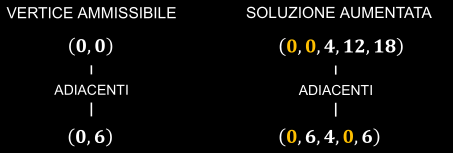
\includegraphics[scale=0.5]{Immagini/Soluzione di base ammissibile_6.png}
    \end{minipage}
    \hfill
    \begin{minipage}{0.45\textwidth}
        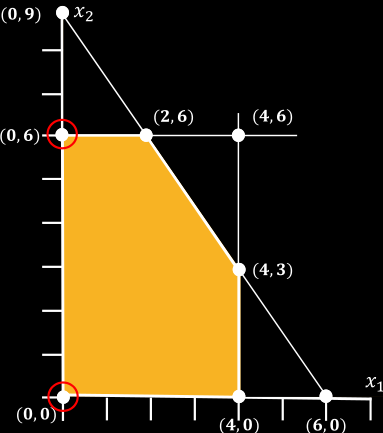
\includegraphics[scale=0.5]{Immagini/Soluzione di base ammissibile_7.png}
    \end{minipage}
\end{center}

Per giungere a questa conclusione non è necessario consultare la figura a destra.

Infatti, un altro indicatore è che le corrispondenti \textbf{variabili non di base} $(\mathbf{x_1},\mathbf{x_2})$ e $(\mathbf{x_1},\mathbf{x_4})$, sono identiche con una sola eccezione $\mathbf{-x_2}$ è rimpiazzata da $\mathbf{x_4}$.

Conseguentemente, muoversi da $(0,0,4,12,18)$ a $(0,6,4,0,6)$ implica che $x_2$ passi dall'essere una \textbf{varabile non di base} ad essere una \textbf{variabile di base}, e che $x_4$ passi dall'essere una \textbf{variabile di base} all'essere una \textbf{variabile non di base}.

\newpage
\section{Procedura algebrica}
\subsection{Intepretazioni}
\subsubsection{Intepretazione geometrica}
\textbf{L'interpretazione geometrica} fa riferimento al \textbf{modello in forma standard (no variabili di slack)} 

\begin{center}
    \begin{minipage}{0.45\textwidth}
        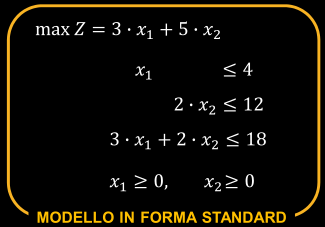
\includegraphics[scale=0.5]{Immagini/Interpretazione geometrica_1.png}
    \end{minipage}
    \hfil
    \begin{minipage}{0.45\textwidth}
        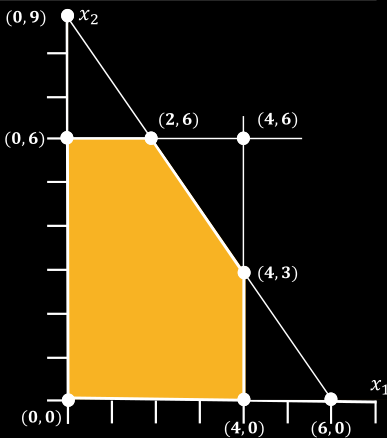
\includegraphics[scale=0.5]{Immagini/Interpretazione geometrica_2.png}
    \end{minipage}
\end{center}

\subsubsection{Intepretazione algebrica}
\textbf{L'interpretazione algebrica} fa riferimento al \textbf{modello in forma aumentata (si variabili slack)}

\begin{center}
    \begin{minipage}{0.45\textwidth}
        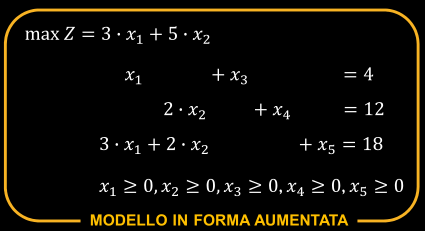
\includegraphics[scale=0.5]{Immagini/Forma algebrica_1.png}
    \end{minipage}
    \hfil
    \begin{minipage}{0.45\textwidth}
        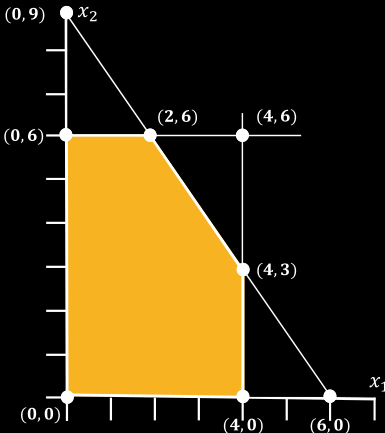
\includegraphics[scale=0.5]{Immagini/Forma algebrica_2.png}
    \end{minipage}
\end{center}

\newpage
\subsection{Inizializzazione}
Scegliere $x_1$ e $x_1$ come variabili non di base (perciò poste a valore nullo) per ottenere la soluzione iniziale di base ammissibile è giustificato dal \textbf{concetto chiave 3}

\begin{center}
    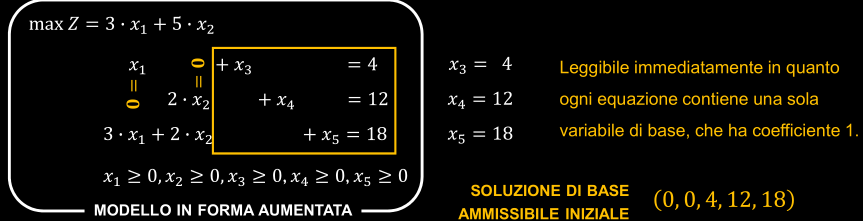
\includegraphics[scale=0.6]{Immagini/Inizializzazione.png}
\end{center}

\subsection{Test di ottimalità}
$x_3,x_4$ e $x_5$ non compaiono nella funzione obiettivo $Z$, per cui sono coefficienti delle variabili non di base, $x_1$ e $x_2$, a determinare il \textbf{tasso di crescità} di $Z$.

I \textbf{tassi di crescita} sono rispettivamente 3 e 4, entrambi positivi.

\begin{center}
    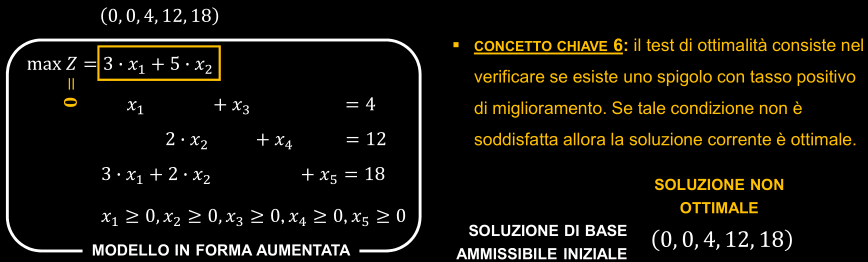
\includegraphics[scale=0.6]{Immagini/Test di ottimalità.png}
\end{center}

\subsection{Passo 1 - Determinazione della direzione di spostamento}
Aumentare il valore di una variabile non di base a partire da zero (modificando i valori di base correnti per soddisfare le equazioni) equivalre a spostarsi lungo uno degli spigoli che emanano dal corrente vertice ammissibile

\begin{center}
    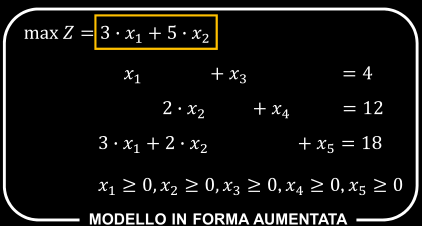
\includegraphics[scale=.6]{Immagini/Determinazione dello spostamento.png}
\end{center}

\newpage
\subsection{Passo 2 - Determinazione dell'incremento}
Determina di quanto aumentare il valore della variabile entrante di base $(x_2)$.

Incrementare il valore di $x_2$ fa incrementare il valore della funzione obiettivo $Z$, pertanto desideriamo aumentare il più possibile il valore di $x_2$ evitando però di abbandonare la regione ammissibile.

Il soddisfacimento dei \textbf{vincoli} implica che se $x_2$ aumentata, mentre si mantiene il valore della variabile non di base $x_1$ uguale a zero, allora il valore di qualche altra variabile di base da variare.

\begin{center}
    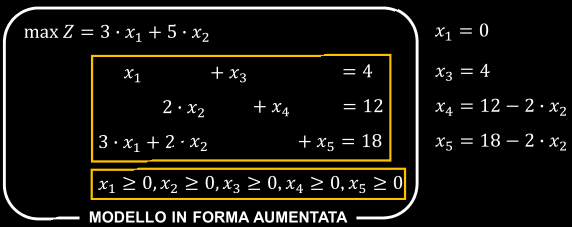
\includegraphics[scale=0.65]{Immagini/Determinazione dell'incremento.png}
\end{center}

L'ammissibilità richiede inoltre che \textbf{tutte le variabili siano non negative}.

Le variabili non di base (inclusa quella entrante $x_2$) sono non negative, ma dobbiamo verificare quanto $x_2$ possa aumentare senza violare il vincolo di non negatività sulle variabili di base $x_3,x_4,x_5$.

\begin{center}
    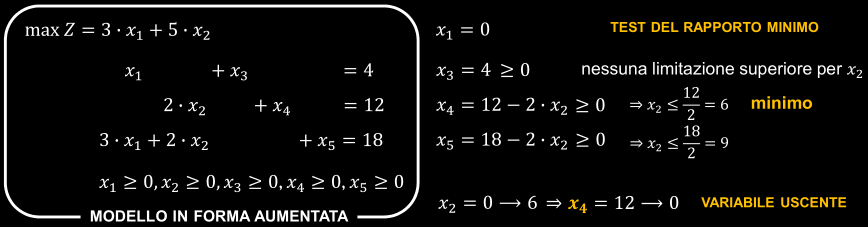
\includegraphics[scale=0.6]{Immagini/incremento_2.png}
\end{center}

Il \textbf{passo 2 dell'algoritmo del simplesso} determina quale variabile di base diminuisce a zero per prima quando si incrementa il valore della \textbf{variabile entrante} in base.

Diminuire il valore della variabile di base fino a raggiungere il valore zero trasforma questa variabile da variabile di base in variabile non di base nella nuova soluzione di base ammissibile. Peranto, questa variabile è chiamata \textbf{variabile uscente} dalla base all'iterazione corrente.

\newpage
\subsection{Passo 3 - Determinazione della nuova soluzione di base}
$x_1$ rimpiazza $x_5$, entrando in base. 

Effetuiamo operazioni algebriche elementari sul \textbf{sistema di equazioni} per riprodurre il pattern $(0,0,0,1)$ di $x_5$ per i nuovi coefficienti di $x_1$.

Questo porta al suguente nuovo sistema di equazioni

\begin{center}
    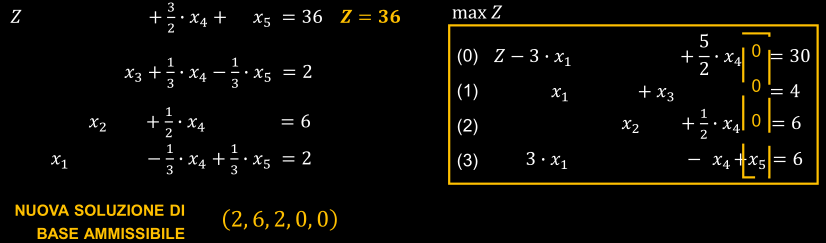
\includegraphics[scale=0.6]{Immagini/Determinazione soluzione di base.png}
    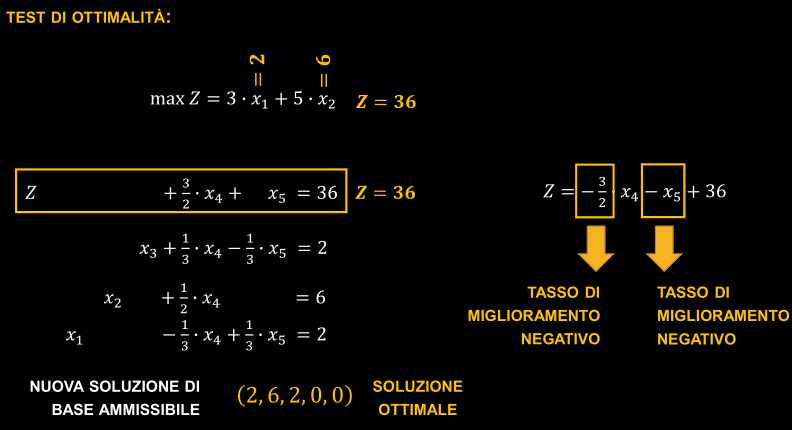
\includegraphics[scale=0.6]{Immagini/Determinazione soluzione di base_2.png}
\end{center}

\newpage
\section{Forma tabellare}
\subsection{Cosa è?}
La forma algebrica è la migliore per comprendere la logica sottostante il metodo del simplesso.

Comunque, la forma algebrica non è la più adeguata per effettuare le computazioni che abbiamo mostrato in precedenza, molto meglio in questo caso utilizzare la \textbf{forma tabellare} che registra solo l'informazione essenziale:

\begin{itemize}
    \item Coefficienti delle variabili
    \item Termini noti delle equazioni
    \item Variabili di base per ogni equazione
\end{itemize}

La \textbf{forma tabellare} evita di memorizzare i simboli delle variabili in ogni equazione, ma cosa ancor più importante è rappresentata dal fatto che, è possibile evidenziare i numeri che sono coinvolti nelle computazioni ed è possibile memorizzare in modo compatto tali numeri

\subsection{Tabella}
\begin{table}[htbp]
\centering
\renewcommand{\arraystretch}{1.3}
\begin{tabular}{l r r r r r r @{\;=\;} r | c | c | c | c c c c c | c}
\hline
\multicolumn{8}{c|}{\textbf{\textsc{Forma Algebrica}}} & \multicolumn{9}{c}{\textbf{\textsc{Forma Tabellare}}} \\
\hline
\multicolumn{8}{c|}{} & \multirow{2}{*}{\shortstack{\textbf{VARIABILE}\\\textbf{DI BASE}}} & & \multicolumn{6}{c|}{\textbf{COEFFICIENTE}} & \multirow{2}{*}{\rotatebox{90}{\shortstack{\textbf{TERMINE}\\\textbf{NOTO}}}} \\
\cline{11-16}
\multicolumn{8}{c|}{} & & \textbf{Eq.} & $\boldsymbol{Z}$ & $\boldsymbol{x_1}$ & $\boldsymbol{x_2}$ & $\boldsymbol{x_3}$ & $\boldsymbol{x_4}$ & $\boldsymbol{x_5}$ & \\[1ex]
\hline
(0) & $\boldsymbol{Z}$ & $- 3x_1$ & $- 5x_2$ & & & & $0$ & $Z$ & (0) & $1$ & $-3$ & $-5$ & $0$ & $0$ & $0$ & $0$ \\
\hline
(1) & & $x_1$ & & $+ \boldsymbol{x_3}$ & & & $4$ & $x_3$ & (1) & $0$ & $1$ & $0$ & $1$ & $0$ & $0$ & $4$ \\
(2) & & & $2x_2$ & & $+ \boldsymbol{x_4}$ & & $12$ & $x_4$ & (2) & $0$ & $0$ & $2$ & $0$ & $1$ & $0$ & $12$ \\
(3) & & $3x_1$ & $+ 2x_2$ & & & $+ \boldsymbol{x_5}$ & $18$ & $x_5$ & (3) & $0$ & $3$ & $2$ & $0$ & $0$ & $1$ & $18$ \\
\hline
\end{tabular}
\end{table}

\newpage
\subsection{Inizializzazione}
Assumendo che il problema sia in \textbf{forma standard}, si procede come segue:
\begin{enumerate}
    \item Aggiungere le variabili slack
    \item Selezionare le variabili di decisione da porre a 0 (non di base)
    \item Selezionare le variabili slack come variabili di base
\end{enumerate}

\begin{table}[htbp]
\centering
\renewcommand{\arraystretch}{1.3}
\begin{NiceTabular}{l r r r r r r @{\;=\;} r | c | c | c | c c c c c | c}
\hline
\multicolumn{8}{c|}{\textbf{\textsc{Forma Algebrica}}} & \multicolumn{9}{c}{\textbf{\textsc{Forma Tabellare}}} \\
\hline
\multicolumn{8}{c|}{} & \multirow{2}{*}{\shortstack{\textbf{VARIABILE}\\\textbf{DI BASE}}} & & \multicolumn{6}{c|}{\textbf{COEFFICIENTE}} & \multirow{2}{*}{\rotatebox{90}{\shortstack{\textbf{TERMINE}\\\textbf{NOTO}}}} \\
\cline{11-16}
\multicolumn{8}{c|}{} & & \textbf{Eq.} & $\boldsymbol{Z}$ & $\boldsymbol{x_1}$ & $\boldsymbol{x_2}$ & $\boldsymbol{x_3}$ & $\boldsymbol{x_4}$ & $\boldsymbol{x_5}$ & \\[1ex]
\hline
(0) & $\boldsymbol{Z}$ & $- 3x_1$ & $- 5x_2$ & & & & $0$ & $Z$ & (0) & $1$ & $-3$ & $-5$ & $0$ & $0$ & $0$ & $0$ \\
(1) & & $x_1$ & & $+ \boldsymbol{x_3}$ & & & $4$ & $x_3$ & (1) & $0$ & $1$ & $0$ & $1$ & $0$ & $0$ & $4$ \\
(2) & & & $2x_2$ & & $+ \boldsymbol{x_4}$ & & $12$ & $x_4$ & (2) & $0$ & $0$ & $2$ & $0$ & $1$ & $0$ & $12$ \\
(3) & & $3x_1$ & $+ 2x_2$ & & & $+ \boldsymbol{x_5}$ & $18$ & $x_5$ & (3) & $0$ & $3$ & $2$ & $0$ & $0$ & $1$ & $18$ \\
\hline
\CodeAfter
  \begin{tikzpicture}
    % Riquadro rosso attorno ai coefficienti e termini noti (righe 4-7, colonne 11-17)
    \draw[red, ultra thick] (4-|11) rectangle (8-|18);
    % Riquadro giallo/arancio attorno alla matrice identità (righe 5-7, colonne 14-16)
    \draw[orange!80!yellow, very thick] ([ shift={(2pt,-1pt)} ] 5-|14) rectangle ([ shift={(-2pt,2pt)} ] 8-|17);
  \end{tikzpicture}
\end{NiceTabular}
\end{table}

\begin{gather*}
    \mathbf{TABLEAU} \\
    x_1=0\ x_2=0 \\
    (0,0,4,12,18) \quad \text{Soluzione di base ammissibile}
\end{gather*}

\subsection{Test di ottimalità}
La \textbf{soluzione di base ammissibile corrente} è ottimale solo se tutti i coefficienti della riga $(0)$ sono non negativi.

Se questo è il caso ci si arresta, altrimenti si effettua un'iterazione per ottenere una nuova soluzione di base ammissibile, il che implica che una variabile non di base venga trasformata in una variabile di base (passo 1) e viceversa (passo 2), per poi ottenere una nuova soluzione (passo 3)

\begin{table}[htbp]
\centering
\renewcommand{\arraystretch}{1.3}
\begin{NiceTabular}{l r r r r r r @{\;=\;} r | c | c | c | c c c c c | c}
\hline
\multicolumn{8}{c|}{\textbf{\textsc{Forma Algebrica}}} & \multicolumn{9}{c}{\textbf{\textsc{Forma Tabellare}}} \\
\hline
\multicolumn{8}{c|}{} & \multirow{2}{*}{\shortstack{\textbf{VARIABILE}\\\textbf{DI BASE}}} & & \multicolumn{6}{c|}{\textbf{COEFFICIENTE}} & \multirow{2}{*}{\rotatebox{90}{\shortstack{\textbf{TERMINE}\\\textbf{NOTO}}}} \\
\cline{11-16}
\multicolumn{8}{c|}{} & & \textbf{Eq.} & $\boldsymbol{Z}$ & $\boldsymbol{x_1}$ & $\boldsymbol{x_2}$ & $\boldsymbol{x_3}$ & $\boldsymbol{x_4}$ & $\boldsymbol{x_5}$ & \\[1ex]
\hline
(0) & $\boldsymbol{Z}$ & $- 3x_1$ & $- 5x_2$ & & & & $0$ & $Z$ & (0) & $1$ & $-3$ & $-5$ & $0$ & $0$ & $0$ & $0$ \\
(1) & & $x_1$ & & $+ \boldsymbol{x_3}$ & & & $4$ & $x_3$ & (1) & $0$ & $1$ & $0$ & $1$ & $0$ & $0$ & $4$ \\
(2) & & & $2x_2$ & & $+ \boldsymbol{x_4}$ & & $12$ & $x_4$ & (2) & $0$ & $0$ & $2$ & $0$ & $1$ & $0$ & $12$ \\
(3) & & $3x_1$ & $+ 2x_2$ & & & $+ \boldsymbol{x_5}$ & $18$ & $x_5$ & (3) & $0$ & $3$ & $2$ & $0$ & $0$ & $1$ & $18$ \\
\hline
\CodeAfter
  \begin{tikzpicture}
    % Riquadro rosso attorno ai coefficienti e termini noti (righe 4-7, colonne 11-17)
    \draw[red, ultra thick] (4-|11) rectangle (8-|18);
    % Riquadro giallo/arancio attorno ai coefficienti di x1..x5 nella riga (0) (riga 4, colonne 12-16)
    \draw[orange!80!yellow, very thick] ([ shift={(2pt,-2pt)} ] 4-|12) rectangle ([ shift={(-2pt,1pt)} ] 5-|17);
  \end{tikzpicture}
\end{NiceTabular}
\end{table}

\subsection{Passo 1}
\begin{enumerate}
    \item Identificare la variabile entrante (selezionandola tra quelle non di base) come quella cui corrisponde il \textbf{minimo coefficiente negativo nell'equazione (0)}
    \item La colonna corrispondente viene identificata tramite un rettangolo e viene denominata \textbf{colonna pivot}
\end{enumerate}

\begin{table}[htbp]
\centering
\renewcommand{\arraystretch}{1.3}
\begin{NiceTabular}{l r r r r r r @{\;=\;} r | c | c | c | c c c c c | c}
\hline
\multicolumn{8}{c|}{\textbf{\textsc{Forma Algebrica}}} & \multicolumn{9}{c}{\textbf{\textsc{Forma Tabellare}}} \\
\hline
\multicolumn{8}{c|}{} & \multirow{2}{*}{\shortstack{\textbf{VARIABILE}\\\textbf{DI BASE}}} & & \multicolumn{6}{c|}{\textbf{COEFFICIENTE}} & \multirow{2}{*}{\rotatebox{90}{\shortstack{\textbf{TERMINE}\\\textbf{NOTO}}}} \\
\cline{11-16}
\multicolumn{8}{c|}{} & & \textbf{Eq.} & $\boldsymbol{Z}$ & $\boldsymbol{x_1}$ & $\boldsymbol{x_2}$ & $\boldsymbol{x_3}$ & $\boldsymbol{x_4}$ & $\boldsymbol{x_5}$ & \\[1ex]
\hline
(0) & $\boldsymbol{Z}$ & $- 3x_1$ & $- 5x_2$ & & & & $0$ & $Z$ & (0) & $1$ & $-3$ & $-5$ & $0$ & $0$ & $0$ & $0$ \\
(1) & & $x_1$ & & $+ \boldsymbol{x_3}$ & & & $4$ & $x_3$ & (1) & $0$ & $1$ & $0$ & $1$ & $0$ & $0$ & $4$ \\
(2) & & & $2x_2$ & & $+ \boldsymbol{x_4}$ & & $12$ & $x_4$ & (2) & $0$ & $0$ & $2$ & $0$ & $1$ & $0$ & $12$ \\
(3) & & $3x_1$ & $+ 2x_2$ & & & $+ \boldsymbol{x_5}$ & $18$ & $x_5$ & (3) & $0$ & $3$ & $2$ & $0$ & $0$ & $1$ & $18$ \\
\hline
\CodeAfter
  \begin{tikzpicture}
    % Riquadro rosso attorno ai coefficienti e termini noti (righe 4-7, colonne 11-17)
    \draw[red, ultra thick] (4-|11) rectangle (8-|18);
    % Riquadro giallo/arancio orizzontale attorno ai coefficienti di x1..x5 nella riga (0)
    \draw[orange!80!yellow, thick] ([ shift={(2pt,-2pt)} ] 4-|12) rectangle ([ shift={(-2pt,1pt)} ] 5-|17);
    % Riquadro giallo/arancio verticale attorno alla colonna pivot x2 (righe 3-7, colonna 13)
    \draw[orange!80!yellow, very thick] ([ shift={(1pt,-2pt)} ] 3-|13) rectangle ([ shift={(-1pt,2pt)} ] 8-|14);
  \end{tikzpicture}
\end{NiceTabular}
\end{table}

\subsection{Passo 2}
Determinare la \textbf{variabile di base uscente} tramite il \textbf{test del rapporto minimo}
\begin{enumerate}
    \item Selezionare i coefficienti strettamente positivi della colonna pivot

    \begin{table}[htbp]
    \centering
    \renewcommand{\arraystretch}{1.4}
    \begin{NiceTabular}{c | c | c | c c c c c | c c}
    \hline
    \multirow{2}{*}{\shortstack{\textbf{VARIABILE}\\\textbf{DI BASE}}} & & \multicolumn{6}{c|}{\textbf{COEFFICIENTE}} & \textbf{TERMINE} & \\
    \cline{3-8}
    & \textbf{Eq.} & $\boldsymbol{Z}$ & $\boldsymbol{x_1}$ & $\boldsymbol{x_2}$ & $\boldsymbol{x_3}$ & $\boldsymbol{x_4}$ & $\boldsymbol{x_5}$ & \textbf{NOTO} & \textbf{RAPPORTO} \\
    \hline
    $Z$ & (0) & $1$ & $-3$ & $-5$ & $0$ & $0$ & $0$ & $0$ & \\
    $x_3$ & (1) & $0$ & $1$ & $0$ & $1$ & $0$ & $0$ & $4$ & \\[1ex]
    $x_4$ & (2) & $0$ & $0$ & $2$ & $0$ & $1$ & $0$ & $12$ & \\[1ex]
    $x_5$ & (3) & $0$ & $3$ & $2$ & $0$ & $0$ & $1$ & $18$ & \\
    \hline
    \CodeAfter
    \begin{tikzpicture}
        % Riquadro giallo/arancio esterno attorno all'intera colonna x2 (righe 2-6, colonna 5)
        \draw[orange!80!yellow, very thick] ([ shift={(-2pt,-2pt)} ] 2-|5) rectangle ([ shift={(2pt,2pt)} ] 7-|6);
        % Riquadro giallo/arancio interno attorno ai coefficienti 2 e 2 (righe 5-6, colonna 5)
        \draw[orange!80!yellow, very thick] ([ shift={(3pt,-2pt)} ] 5-|5) rectangle ([ shift={(-3pt,4pt)} ] 7-|6);
    \end{tikzpicture}
    \end{NiceTabular}
    \end{table}

    \item Dividere i termini noti per questi coefficienti (riga omologa)

    \begin{table}[htbp]
    \centering
    \renewcommand{\arraystretch}{1.4}
    \begin{NiceTabular}{c | c | c | c c c c c | c c c}
    \hline
    \multirow{2}{*}{\shortstack{\textbf{VARIABILE}\\\textbf{DI BASE}}} & & \multicolumn{6}{c|}{\textbf{COEFFICIENTE}} & \textbf{TERMINE} & & \\
    \cline{3-8}
    & \textbf{Eq.} & $\boldsymbol{Z}$ & $\boldsymbol{x_1}$ & $\boldsymbol{x_2}$ & $\boldsymbol{x_3}$ & $\boldsymbol{x_4}$ & $\boldsymbol{x_5}$ & \textbf{NOTO} & & \textbf{RAPPORTO} \\
    \hline
    $Z$ & (0) & $1$ & $-3$ & $-5$ & $0$ & $0$ & $0$ & $0$ & & \\
    $x_3$ & (1) & $0$ & $1$ & $0$ & $1$ & $0$ & $0$ & $4$ & & \\[1.5ex]
    $x_4$ & (2) & $0$ & $0$ & $2$ & $0$ & $1$ & $0$ & $12$ & $\rightarrow \dfrac{12}{2}$ & \\[2.5ex]
    $x_5$ & (3) & $0$ & $3$ & $2$ & $0$ & $0$ & $1$ & $18$ & $\rightarrow \dfrac{18}{2}$ & \\[1ex]
    \hline
    \CodeAfter
    \begin{tikzpicture}
        % Riquadro giallo/arancio attorno ai coefficienti 2 e 2 di x2 (righe 5-6, colonna 5)
        \draw[orange!80!yellow, very thick] ([ shift={(3pt,-2pt)} ] 5-|5) rectangle ([ shift={(-3pt,4pt)} ] 7-|6);
        % Riquadro giallo/arancio attorno ai termini noti e alle frazioni (righe 5-6, colonne 9-10)
        \draw[orange!80!yellow, very thick] ([ shift={(2pt,-4pt)} ] 5-|9) rectangle ([ shift={(-2pt,4pt)} ] 7-|11);
    \end{tikzpicture}
    \end{NiceTabular}
    \end{table}

    \newpage
    \item Selezionare la riga cui corrisponde il più piccolo rapporto calcolato al punto 2

    \begin{table}[htbp]
    \centering
    \renewcommand{\arraystretch}{1.4}
    \begin{NiceTabular}{c | c | c | c c c c c | c @{\;} r @{\;} c @{\;} l}
    \hline
    \multirow{2}{*}{\shortstack{\textbf{VARIABILE}\\\textbf{DI BASE}}} & & \multicolumn{6}{c|}{\textbf{COEFFICIENTE}} & \textbf{TERMINE} & \multicolumn{3}{c}{} \\
    \cline{3-8}
    & \textbf{Eq.} & $\boldsymbol{Z}$ & $\boldsymbol{x_1}$ & $\boldsymbol{x_2}$ & $\boldsymbol{x_3}$ & $\boldsymbol{x_4}$ & $\boldsymbol{x_5}$ & \textbf{NOTO} & \multicolumn{3}{c}{\textbf{RAPPORTO}} \\
    \hline
    $Z$ & (0) & $1$ & $-3$ & $-5$ & $0$ & $0$ & $0$ & $0$ & & & \\
    $x_3$ & (1) & $0$ & $1$ & $0$ & $1$ & $0$ & $0$ & $4$ & & & \\[1.5ex]
    $x_4$ & (2) & $0$ & $0$ & $2$ & $0$ & $1$ & $0$ & $12$ & $\rightarrow \dfrac{12}{2} =$ & $6$ & $\leftarrow \text{minimum}$ \\[2.5ex]
    $x_5$ & (3) & $0$ & $3$ & $2$ & $0$ & $0$ & $1$ & $18$ & $\rightarrow \dfrac{18}{2} =$ & $9$ & \\[1ex]
    \hline
    \CodeAfter
    \begin{tikzpicture}
        % Riquadro giallo/arancio verticale attorno ai risultati dei rapporti 6 e 9 (righe 5-6, colonna 11)
        \draw[orange!80!yellow, very thick] ([ shift={(-2pt,-4pt)} ] 5-|11) rectangle ([ shift={(2pt,4pt)} ] 7-|12);
        % Riquadro giallo/arancio attorno alla parola "minimum" (riga 5, colonna 12)
        \draw[orange!80!yellow, very thick] ([ shift={(13pt,-6pt)} ] 5-|12) rectangle ([ shift={(2pt,9pt)} ] 6-|13);
    \end{tikzpicture}
    \end{NiceTabular}
    \end{table}

    \item La variabile di base di quella riga è la variabile di base uscente, rimpiazzarla con la variabile entrante

    \begin{table}[htbp]
    \centering
    \renewcommand{\arraystretch}{1.4}
    \begin{NiceTabular}{c | c | c | c c c c c | c @{\;} r @{\;} c @{\;} l}
    \hline
    \multirow{2}{*}{\shortstack{\textbf{VARIABILE}\\\textbf{DI BASE}}} & & \multicolumn{6}{c|}{\textbf{COEFFICIENTE}} & \textbf{TERMINE} & \multicolumn{3}{c}{} \\
    \cline{3-8}
    & \textbf{Eq.} & $\boldsymbol{Z}$ & $\boldsymbol{x_1}$ & $\boldsymbol{x_2}$ & $\boldsymbol{x_3}$ & $\boldsymbol{x_4}$ & $\boldsymbol{x_5}$ & \textbf{NOTO} & \multicolumn{3}{c}{\textbf{RAPPORTO}} \\
    \hline
    $Z$ & (0) & $1$ & $-3$ & $-5$ & $0$ & $0$ & $0$ & $0$ & & & \\
    $x_3$ & (1) & $0$ & $1$ & $0$ & $1$ & $0$ & $0$ & $4$ & & & \\[1.5ex]
    $x_4$ & (2) & $0$ & $0$ & $2$ & $0$ & $1$ & $0$ & $12$ & $\rightarrow \dfrac{12}{2} =$ & $6$ & $\leftarrow \text{minimum}$ \\[2.5ex]
    $x_5$ & (3) & $0$ & $3$ & $2$ & $0$ & $0$ & $1$ & $18$ & $\rightarrow \dfrac{18}{2} =$ & $9$ & \\[1ex]
    \hline
    \CodeAfter
    \begin{tikzpicture}
        % Riquadro giallo/arancio verticale attorno alla colonna pivot x2 (righe 2-6, colonna 5)
        \draw[orange!80!yellow, very thick] ([ shift={(1pt,-2pt)} ] 2-|5) rectangle ([ shift={(-1pt,4pt)} ] 7-|6);
        % Riquadro giallo/arancio orizzontale attorno alla riga pivot (2) da x4 fino a x5 (riga 5, colonne 1-8)
        \draw[orange!80!yellow, very thick] ([ shift={(4pt,-3pt)} ] 5-|1) rectangle ([ shift={(-4pt,8pt)} ] 6-|9);
    \end{tikzpicture}
    \end{NiceTabular}
    \end{table}

\end{enumerate}

\subsection{Passo 3}
Determinare la \textbf{nuova soluzione di base} applicando operazioni che consentano l'uso dell'\textbf{eliminazione Gaussiana}

\begin{enumerate}
    \item Dividere la riga pivot per il numero pivot, ottenendo un nuovo numero pivot ed una nuova riga pivot

    \begin{table}[htbp]
    \centering
    \renewcommand{\arraystretch}{1.35}
    \begin{NiceTabular}{c c | c | c | c c c c c | r}
    \hline
    & \multirow{2}{*}{\shortstack{\textbf{VARIABILE}\\\textbf{DI BASE}}} & & \multicolumn{6}{c|}{\textbf{COEFFICIENTE}} & \textbf{TERMINE} \\
    \cline{4-9}
    \textbf{ITERAZIONE} & & \textbf{Eq.} & $\boldsymbol{Z}$ & $\boldsymbol{x_1}$ & $\boldsymbol{x_2}$ & $\boldsymbol{x_3}$ & $\boldsymbol{x_4}$ & $\boldsymbol{x_5}$ & \multicolumn{1}{c}{\textbf{NOTO}} \\
    \hline
    \multirow{4}{*}{0} & $Z$ & (0) & $1$ & $-3$ & $-5$ & $0$ & $0$ & $0$ & $0$ \\
    & $x_3$ & (1) & $0$ & $1$ & $0$ & $1$ & $0$ & $0$ & $4$ \\
    & $x_4$ & (2) & $0$ & $0$ & $2$ & $0$ & $1$ & $0$ & $12$ \\
    & $x_5$ & (3) & $0$ & $3$ & $2$ & $0$ & $0$ & $1$ & $18$ \\
    \hline
    \multirow{4}{*}{1} & $Z$ & (0) & $1$ & & & & & & \\
    & $x_3$ & (1) & $0$ & & & & & & \\[0.5ex]
    & $x_2$ & (2) & $0$ & $0$ & $1$ & $0$ & $\dfrac{1}{2}$ & $0$ & $6$ \\[1ex]
    & $x_5$ & (3) & $0$ & & & & & & \\
    \hline
    \CodeAfter
    \begin{tikzpicture}
        % Riquadro giallo/arancio attorno alla colonna x2 nell'iterazione 0 (righe 2-6, colonna 6)
        \draw[orange!80!yellow, very thick] ([ shift={(1pt,-2pt)} ] 2-|6) rectangle ([ shift={(-1pt,2pt)} ] 7-|7);
        % Riquadro rosso attorno alla colonna x4 nell'iterazione 0 (righe 2-6, colonna 8)
        \draw[red, very thick] ([ shift={(1pt,-2pt)} ] 2-|8) rectangle ([ shift={(-1pt,2pt)} ] 7-|9);
        % Riquadro verde attorno alla riga (2) nell'iterazione 0 (riga 5, colonne 5-10)
        \draw[green!65!black, very thick] ([ shift={(2pt,-1pt)} ] 5-|5) rectangle ([ shift={(-2pt,2pt)} ] 6-|11);
        % Riquadro verde attorno alla nuova riga (2) nell'iterazione 1 (riga 9, colonne 5-10)
        \draw[green!65!black, very thick] ([ shift={(2pt,-3pt)} ] 9-|5) rectangle ([ shift={(-2pt,3pt)} ] 10-|11);
    \end{tikzpicture}
    \end{NiceTabular}
    \end{table}

    \item Ad ogni altra riga (inclusa la riga 0) che abbia coefficiente negativo nella colonna pivot, sommare a questa riga il prodotto del valore assoluto del coefficiente per la nuova riga pivot

    \begin{table}[htbp]
    \centering
    \renewcommand{\arraystretch}{1.35}
    \begin{NiceTabular}{c c | c | c | c c c c c | r}
    \hline
    & \multirow{2}{*}{\shortstack{\textbf{VARIABILE}\\\textbf{DI BASE}}} & & \multicolumn{6}{c|}{\textbf{COEFFICIENTE}} & \textbf{TERMINE} \\
    \cline{4-9}
    \textbf{ITERAZIONE} & & \textbf{Eq.} & $\boldsymbol{Z}$ & $\boldsymbol{x_1}$ & $\boldsymbol{x_2}$ & $\boldsymbol{x_3}$ & $\boldsymbol{x_4}$ & $\boldsymbol{x_5}$ & \multicolumn{1}{c}{\textbf{NOTO}} \\
    \hline
    \multirow{4}{*}{0} & $Z$ & (0) & $1$ & $-3$ & $-5$ & $0$ & $0$ & $0$ & $0$ \\
    & $x_3$ & (1) & $0$ & $1$ & $0$ & $1$ & $0$ & $0$ & $4$ \\
    & $x_4$ & (2) & $0$ & $0$ & $2$ & $0$ & $1$ & $0$ & $12$ \\
    & $x_5$ & (3) & $0$ & $3$ & $2$ & $0$ & $0$ & $1$ & $18$ \\
    \hline
    \multirow{4}{*}{1} & $Z$ & (0) & $1$ & $-3$ & $0$ & $0$ & $\dfrac{5}{2}$ & $0$ & $30$ \\[1ex]
    & $x_3$ & (1) & $0$ & & & & & & \\[0.5ex]
    & $x_2$ & (2) & $0$ & $0$ & $1$ & $0$ & $\dfrac{1}{2}$ & $0$ & $6$ \\[1ex]
    & $x_5$ & (3) & $0$ & & & & & & \\
    \hline
    \CodeAfter
    \begin{tikzpicture}
        % Riquadri grigi verticali attorno alle colonne x2 e x4 nell'iterazione 0 (righe 2-6)
        \draw[gray!80, very thick] ([ shift={(1pt,-2pt)} ] 2-|6) rectangle ([ shift={(-1pt,2pt)} ] 7-|7);
        \draw[gray!80, very thick] ([ shift={(1pt,-2pt)} ] 2-|8) rectangle ([ shift={(-1pt,2pt)} ] 7-|9);
        % Riquadro verde attorno alla riga (0) nell'iterazione 0 (riga 3, colonne 5-10)
        \draw[green!65!black, very thick] ([ shift={(2pt,-2pt)} ] 3-|5) rectangle ([ shift={(-2pt,2pt)} ] 4-|11);
        % Riquadro verde attorno alla nuova riga (0) nell'iterazione 1 (riga 7, colonne 5-10)
        \draw[green!65!black, very thick] ([ shift={(2pt,-2pt)} ] 7-|5) rectangle ([ shift={(-2pt,2pt)} ] 8-|11);
        % Riquadro giallo/arancio attorno alla riga pivot (2) nell'iterazione 1 (riga 9, colonne 5-10)
        \draw[orange!80!yellow, very thick] ([ shift={(2pt,-3pt)} ] 9-|5) rectangle ([ shift={(-2pt,3pt)} ] 10-|11);
    \end{tikzpicture}
    \end{NiceTabular}
    \end{table}

    \item Ad ogni altra riga (inclusa la riga 0) che abbia coefficiente positivo nella colonna pivot, sottrarre a questa riga il prodotto del valore assoluto del coefficiente per la nuova riga pivot

    \begin{table}[htbp]
    \centering
    \renewcommand{\arraystretch}{1.35}
    \begin{NiceTabular}{c c | c | c | c c c c c | r}
    \hline
    & \multirow{2}{*}{\shortstack{\textbf{VARIABILE}\\\textbf{DI BASE}}} & & \multicolumn{6}{c|}{\textbf{COEFFICIENTE}} & \textbf{TERMINE} \\
    \cline{4-9}
    \textbf{ITERAZIONE} & & \textbf{Eq.} & $\boldsymbol{Z}$ & $\boldsymbol{x_1}$ & $\boldsymbol{x_2}$ & $\boldsymbol{x_3}$ & $\boldsymbol{x_4}$ & $\boldsymbol{x_5}$ & \multicolumn{1}{c}{\textbf{NOTO}} \\
    \hline
    \multirow{4}{*}{0} & $Z$ & (0) & $1$ & $-3$ & $-5$ & $0$ & $0$ & $0$ & $0$ \\
    & $x_3$ & (1) & $0$ & $1$ & $0$ & $1$ & $0$ & $0$ & $4$ \\
    & $x_4$ & (2) & $0$ & $0$ & $2$ & $0$ & $1$ & $0$ & $12$ \\
    & $x_5$ & (3) & $0$ & $3$ & $2$ & $0$ & $0$ & $1$ & $18$ \\
    \hline
    \multirow{4}{*}{1} & $Z$ & (0) & $1$ & $-3$ & $0$ & $0$ & $\dfrac{5}{2}$ & $0$ & $30$ \\[1ex]
    & $x_3$ & (1) & $0$ & & & & & & \\[0.5ex]
    & $x_2$ & (2) & $0$ & $0$ & $1$ & $0$ & $\dfrac{1}{2}$ & $0$ & $6$ \\[1ex]
    & $x_5$ & (3) & $0$ & $3$ & $0$ & $0$ & $-1$ & $1$ & $6$ \\
    \hline
    \CodeAfter
    \begin{tikzpicture}
        % Riquadri grigi verticali attorno alle colonne x2 e x4 nell'iterazione 0 (righe 2-6)
        \draw[gray!80, very thick] ([ shift={(1pt,-2pt)} ] 2-|6) rectangle ([ shift={(-1pt,2pt)} ] 7-|7);
        \draw[gray!80, very thick] ([ shift={(1pt,-2pt)} ] 2-|8) rectangle ([ shift={(-1pt,2pt)} ] 7-|9);
        % Riquadro verde attorno alla riga (3) nell'iterazione 0 (riga 6, colonne 5-10)
        \draw[green!65!black, very thick] ([ shift={(2pt,-1pt)} ] 6-|5) rectangle ([ shift={(-2pt,2pt)} ] 7-|11);
        % Riquadro giallo/arancio attorno alla riga pivot (2) nell'iterazione 1 (riga 9, colonne 5-10)
        \draw[orange!80!yellow, very thick] ([ shift={(2pt,-3pt)} ] 9-|5) rectangle ([ shift={(-2pt,3pt)} ] 10-|11);
    \end{tikzpicture}
    \end{NiceTabular}
    \end{table}
\end{enumerate}

\newpage
\section{Tie Breaking}